\chapter{Chosen Index Structures}
\label{chap:chosen-structures}
\vspace{-0.75cm}
\centerline{\rule{149mm}{.02in}}
\vspace{0.75cm}

Six index structures will be implemented and evaluated in this report. These structures are sequential scan, PR octree, Pseudo-Pyramid Tree, Pyramid Tree, Bit Hash and the point $kd$-tree. This section will describe these structures in detail and discuss the reasons for choosing them.

\section{Baselines}
\label{sec:baselines}

There is little use in measuring the performance of the implemented index structures if there is nothing to compare the results to. Two baseline structures have been chosen: sequential scan and the PR octree (see Sections \ref{sec:basic-structures} and \ref{sec:recursive-partition-structures} respectively).

Sequential scan has been chosen as a baseline because it is the na\"{i}ve brute-force approach to performing search. The PR octree was chosen because it is the basis of many index structures, both old and new. Both of these structures are well-known in the field, making them suitable baselines.

\section{Pyramid Tree}
\label{sec:pyramid-tree-detail}

As described in Section \ref{sec:high-dimensional-structures}, the pyramid tree reduces multi-dimensional points to one dimension, which can then be used in a one-dimensional index structure. The reason this structure has been chosen is because dimension reduction techniques have been found to perform well for high-dimensional data, compared to tree-based approaches \cite{md-structures-samet}. The original Pyramid-Tree paper showed good performance on uniformly distributed data and a real dataset (with the Extended Pyramid-Technique), when compared to Sequential Scan and the competitive X-tree \cite{pyramid-tree}. There are two fundamental differences between the focus of the paper's analysis and what this project is trying to achieve:
\begin{enumerate}
	\item the paper's analysis is for \textit{range} queries, whereas this project is focused on point queries
	\item the real dataset, ``a large text database extracted from WWW-pages" \cite{pyramid-tree}, contains discrete values, whereas the real datasets considered in this project are continuous, scientific datasets
\end{enumerate}
While the database is mapped to a spatial domain when stored in an index structure, the data may have different properties or distributions than continuous, spatial-based data. Scientific datasets, the target of this project, tend to model continuous domains. Therefore, it was decided that the Pyramid Tree will be implemented to explore if the structure can provide equally good performance with point queries on dynamic scientific datasets.

The dimension reduction technique will now be explained in further detail. The Pyramid tree partitions the data space into $2d$ Pyramids, where each pyramid uses a $(d - 1)$ hyperplane for its base and the centre of the data space as its tip. Figure \ref{fig:pyramid-tree-pyramids} shows how the $2d$ pyramids extend from the centre point to the data space's boundaries. Each pyramid is segmented by splitting them along $(d-1)$ hyperplanes parallel to the base of the pyramid.

The one-dimensional value of a point, called the \textit{pyramid value}, defines which pyramid it is in and its height in said pyramid. The resultant spatial partition is shown in Figure \ref{fig:pyramid-tree-buckets}, where each pyramid segment has a bucket that stores the points inside that segment.

\begin{figure}
		\begin{center}
			\begin{subfloat}[$2d$ Pyramids in 2D Data Space\label{fig:pyramid-tree-pyramids}]{%
				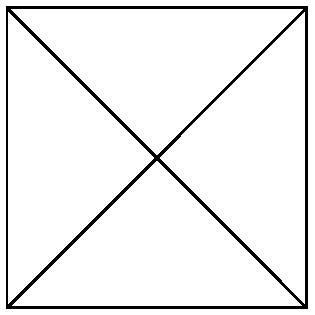
\includegraphics[scale=0.7]{figures/pyramid_tree_partition.pdf}
			}
			\end{subfloat}~~~~
			\begin{subfloat}[Segmented $2d$ Pyramids, Each Associated with a Bucket\label{fig:pyramid-tree-buckets}] {%
				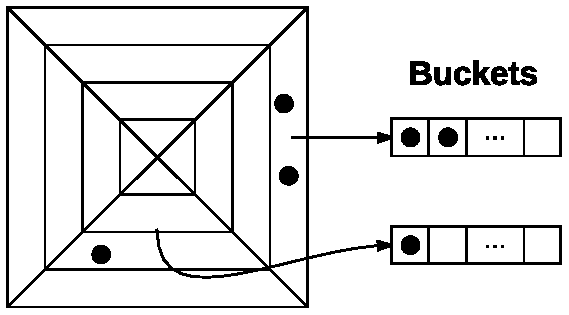
\includegraphics[scale=0.7]{figures/pyramid_tree_buckets.pdf}
			}
			\end{subfloat}
		\end{center}

		\caption{Pyramid Tree's Decomposition of Underlying Data Space}
		\label{fig:pyramid-tree-partition}
\end{figure}

More formally, the pyramid value $pv_v$ of a point $v$ is given by $pv_v = (i + h_v)$, where $i$ represents the pyramid $v$ is contained in, and $h_v$ is height of $v$ in pyramid $i$. $i$ and $h_v$ are given in Equations \ref{eq:pyramid-value-index} and \ref{eq:pyramid-value-height} respectively, where $MOD$ refers to the modulo operator.
\begin{align}
	i &= \begin{cases}
		j_{max},         & \text{if }v_{j_{max}} < 0.5\\
		j_{max} + d,   & \text{if }v_{j_{max}} \geq 0.5\\
	\end{cases}
	\label{eq:pyramid-value-index}
	\\
	j_{max} &= \left( j \;|\; \forall k \; 0 \leq j,k \leq d, j \neq k: \;\; \lvert 0.5 - v_j \rvert \geq \lvert 0.5 - v_k \rvert \right) \nonumber
\end{align}
\begin{equation}
	h_v = \lvert 0.5 - v_{i \; MOD \; d} \rvert
	\label{eq:pyramid-value-height}
\end{equation}

The following lemma shows that two distinct points can be mapped to the same pyramid value. It follows that multiple points may be stored in the same bucket. As such, bucket size will be a key performance factor for the structure and will be measured alongside execution time.

\vspace{22pt}

\begin{proof}[\textbf{Lemma: } For $d \geq 2$, there exist two points $x$ and $y$, such that $x \neq y$, with the same pyramid value]\mbox{}\\*
Let $d$ be the number of dimensions and $x = (x_0, x_1, \dots, x_{d -1})$, $y = (y_0, y_1, \dots, y_{d - 1})$ be two $d$-dimensional points. Without loss of generality, assume $0 \leq x_i \leq 1$ and $0 \leq y_i \leq 1$ for all $i = 1, 2, \dots, d$. Suppose $x_0 = y_0 = 0$, $x_{d - 1} = 0.1$, $y_{d - 1} = 0.2$ and $x_i = y_i = 0.1$ for all $i = 1, \dots, {d - 2}$. This means $x \neq y$. The following holds:
\begin{enumerate}
	\item $\forall k \; 0 \leq k \leq d, k \neq 0: \;\; \lvert 0.5 - x_0 \rvert \geq \lvert 0.5 - x_k \rvert$,
	\item $\forall k \; 0 \leq k \leq d, k \neq 0: \;\; \lvert 0.5 - y_0 \rvert \geq \lvert 0.5 - y_k \rvert$.
\end{enumerate}
Since $x_0 \leq 0.5$ and $y_0 \leq 0.5$, both $x$ and $y$ are mapped to pyramid 0 ($i = 0$). It follows that $h_x = h_y = \lvert 0.5 - v_{0 \; MOD \; d} \rvert = \lvert 0.5 - v_{0} \rvert = \lvert 0.5 - 0 \rvert = 0.5$. $pv_x = pv_y = 0 + 0.5 = 0.5$ and $x \neq y$, meaning two distinct points can have the same Pyramid value.

\end{proof}

\section{Pseudo-Pyramid Tree}

\begin{wrapfigure}[12]{r}{0.4\textwidth}
	\vspace{-5pt}
	\begin{center}
		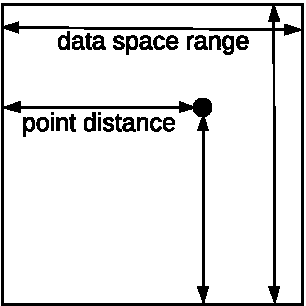
\includegraphics[scale=0.7]{figures/pseudo-pyramid_tree_point_boundary_distances.pdf}
	\end{center}
	\vspace{-15pt}
	\caption{Distance of Point From Data Space Boundaries}
	\label{fig:point-boundary-distance}
\end{wrapfigure}

School of Computing at the University of Leeds have an implementation of an index structure which is similar to the Pyramid Tree. Like the Pyramid Tree, it reduces $d$-dimensional points to a single dimension, which is used to search for the original point in a one-dimensional search structure. Each 1D key has its own bucket that contains references to the original points which are mapped to it. This index structure will be called the \textbf{Pseudo-Pyramid Tree}, because the reduction technique used is \textit{inspired} by the Pyramid tree, but is not the same.  To gain more insight into the performance of dimension reduction techniques as a whole, the Pseudo-Pyramid Tree will be implemented.

The Pseudo-Pyramid Tree reduction will now be given. To reduce a point $p$, how far along the boundary the point is in each dimension is determined (see Figure \ref{fig:point-boundary-distance} for an illustration). These distances are computed using Equation \ref{eq:point-boundary-distance}, where  $min_i$ and $max_i$ define the minimum and maximum bounds for dimension $i$.

\begin{equation}
	h_i(p) = \frac{p_i - min_i}{max_i - min_i}
	\label{eq:point-boundary-distance}
\end{equation}

Let $B$ be a parameter which controls how likely points will be in the same bucket and let $M = \ceil{B^{\frac{1}{d}}}$. The hashed value $h(p)$ of a point $p$ is then given by Equation \ref{eq:pseudo-pyramid-hash}. The function takes $O(d)$ time to compute because of the summation.

\begin{equation}
	h(p) = \sum_{i = 0}^{d} { \lfloor h_i(p) \times M^{i} \rfloor }
	\label{eq:pseudo-pyramid-hash}
\end{equation}

The coefficient $M$ is used to increase the magnitude of $h_i(p)$ before it is truncated with the floor function. This spaces out the mappings of points, decreasing the likelihood two distinct points will be reduced to the same value (and be stored in the same bucket). Increasing $B$ will increase $M$ because $M$ is a power of $B$. Therefore, $B$ can be used to increase or decrease discrimination between points.

\section{Bit Hash}
\label{sec:bit-hash}

% http://stackoverflow.com/questions/7403210/hashing-floating-point-values
% https://svn.boost.org/trac/boost/ticket/4038
% http://programmers.stackexchange.com/questions/63595/0x9e3779b9-golden-number
% http://stackoverflow.com/questions/4948780/magic-number-in-boosthash-combine
% http://burtleburtle.net/bob/hash/doobs.html

Bit Hash is another structure which reduces the dimensionality of points to one dimension. Instead of using a point's spatial properties, Bit Hash accumulates a hash value by hashing each individual coordinate. Each coordinate is hashed using a  32-bit floating point hashing function. The algorithms used for hashing a point and 32-bit floating point numbers are given in Appendix \ref{chap:algs-and-code}.

The structure is susceptible to floating point inaccuracy because it uses the \textit{bits} of the point to produce the hash value. On the controlled performance tests executed in this project, a point is queried using the exact same floating point values for the coordinates as when it was inserted. This means the two points have the same identical bit patterns and these errors will not occur.

Suppose the point being queried was the output of some other computation, where rounding errors may come into play. Even if the point is \textit{mathematically} identical to a point stored in the structure, rounding errors can cause the two points to have different bit patterns and thus, have different hashed values.  Despite the point being stored in the structure, it will appear as if it is not. 

This makes Bit Hash unreliable for certain applications, especially ones where the input points are the result of computations involving many arithmetic operations. Nevertheless, For the small subset of applications where all the points are pre-loaded into memory and not computed again, this can be a useful structure. Initial experiments have also shown this structure has good point query performance, so it will be explored further in this project.

\section{Point $kd$-Tree}
\label{sec:kd-tree-detail}

The $kd$-tree is a widely used structure for both low and high dimensional data. In the literature, there is a lot of discussion as to how and why this structure performs poorly in a high-dimensional setting \cite{highd-nn, search-highd-analysis}. $kd$-trees are typically used for \textit{approximate} queries in higher-dimensional space, because they degenerate to Sequential Scan for exact range and nearest neighbour queries \cite{similarity-searching}. 

Similar to the Pyramid Tree, the focus of the literature on $kd$-trees is typically for range and nearest neighbour queries, and not point queries. Unlike the Pyramid Tree however, dynamic variants of $kd$-trees have been explored much more (e.g. in \cite{bkd-tree, kdb-tree}), with the original paper proposing operations for incremental insertion and removal \cite{kd-tree}. Assessing the suitability of multiple classes of structures provides a more comprehensive evaluation. The $kd$-tree has been chosen because it belongs to a different class of index structure than the other chosen structures, which use dimension reduction.

The structure is a multi-dimensional binary tree, meaning the number of nodes does not increase exponentially with $d$ like the octree. Instead of splitting by all dimensions at each level, $kd$-trees split the data space along a single dimension, called the \textit{cutting dimension}.

The variant of the tree implemented for this project is the point $kd$-tree (Section \ref{sec:recursive-partition-structures}). The cutting dimension at each level is chosen by cycling through the dimensions. If $n$ is a $kd$-tree node, $i$ is the cutting dimension on that node's level and $p$ is the point stored in this node, then:
\begin{enumerate}
	\item Let $q$ be any point in the left subtree rooted at $n$: $p_i > q_i$ holds
	\item Let $q$ be any point in the right subtree rooted at $n$: $p_i \leq q_i$ holds
\end{enumerate}
When inserting or querying a point $p$, the tree is traversed top-down in a similar fashion to a standard binary tree, by comparing $p_i$ to $q_i$, where $q$ is the point stored in the current node and $i$ is the cutting dimension of the current level.

The \texttt{delete} operation used is described in \cite{kdtree-remove}. Relative to \texttt{insert} and point queries, this operation requires more computation because it has to maintain the $kd$-tree invariant. To remove a point $p$, first the node containing $p$ is found using the aforementioned top-down traversal approach. Let $n$ be this node and $i$ be the current level's cutting dimension. If $n$ is a leaf, then the node can simply be deleted. Otherwise, let $n_L$ and $n_R$ be the left and right children of $n$ respectively. 

If $n_R$ exists, a node $m$ containing a point with the \textit{minimum} value for dimension $i$ is found in the sub-tree rooted at $n_R$. The points stored in nodes $n$ and $m$ are swapped and \texttt{delete($p$)} is called recursively on the sub-tree rooted at $n_R$.

If $n_R$ does not exist, node $m$ is found in the sub-tree rooted at $n_L$ instead. In this case, after \texttt{delete($p$)} has been recursively called on the sub-tree rooted at $n_L$, the $i$th value of all points stored in this sub-tree are greater than or equal to the $i$th value of the new point in $n$. Therefore, $n_L$ then becomes the \textit{right} child of $n$ to maintain the $kd$-tree invariant. 

Figure \ref{fig:kd-tree} illustrates the \texttt{insert} and \texttt{delete} operations.

\begin{figure}
	\begin{center}
		\makebox[\textwidth][c]{
		\begin{subfloat}[Inserting Point $(3, 1)$\label{fig:kdtree-insert}]{%
			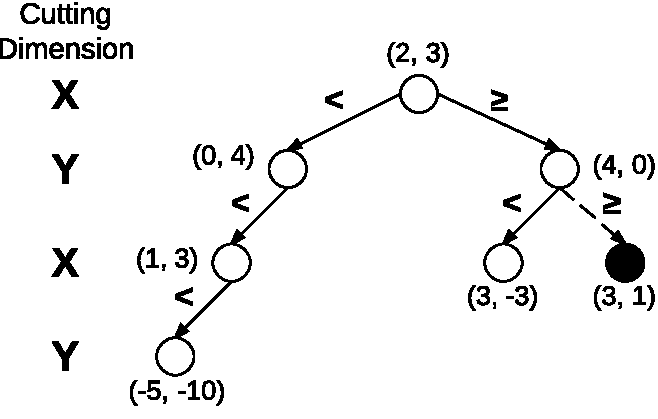
\includegraphics[scale=0.5]{figures/kdtree_insert.pdf}
		}
		\end{subfloat}~~~~
		\begin{subfloat}[Deleting Point $(0, 4)$\label{fig:kdtree-delete}]{%
			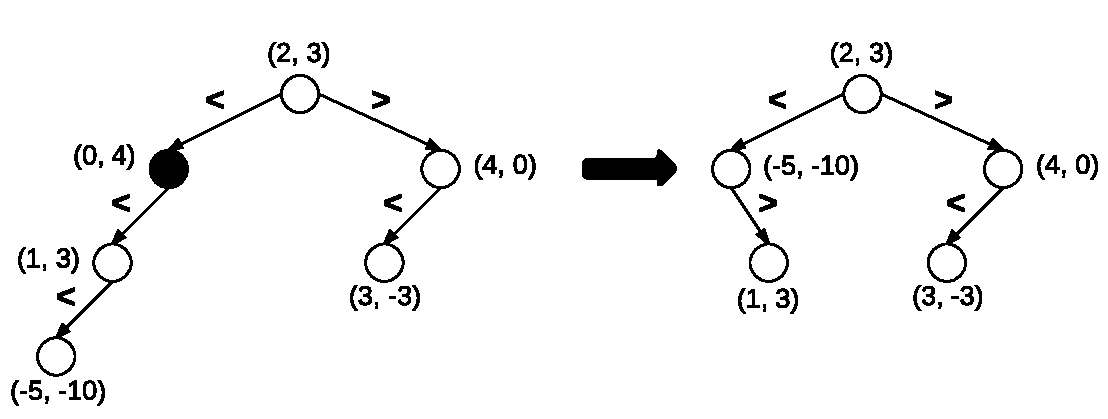
\includegraphics[scale=0.5]{figures/kdtree_delete.pdf}
		}
		\end{subfloat}	  
		}%
	\end{center}

	\caption{$kd$-tree Operations for 2D Dataset (Cutting Dimension Alternates Between X and Y)}
	\label{fig:kd-tree}
\end{figure}